%%%%% Single page layout:
%%%%% ----------------------------------------------------
\documentclass[12pt,a4paper,paper=a4,oneside,titlepage,pdftex]{scrartcl} 

%%% Additional useful packages
%%% ----------------------------------------------------------------
\usepackage{amsmath,amssymb,amsfonts}
\usepackage{algorithmic}
\usepackage{graphicx}
\usepackage{listings}                
\usepackage{graphicx}
\usepackage{subcaption}
\usepackage{float}
\usepackage[utf8]{inputenc}
\usepackage{booktabs}
\usepackage{pdfpages}
\usepackage{hyperref}
\usepackage{url}
\usepackage{color} %red, green, blue, yellow, cyan, magenta, black, white
\usepackage{lipsum}

\begin{document}
	
\pagenumbering{arabic}

\title{Project Report: Users' satisfaction about Dalarna University's Homepage}
\subtitle{ST3012 Data Collection}
\author{
	\bfseries\Large Authors: Péter Tempfli, Tobias Weiß\\
	\{v19pette, v18tobwe\}@du.se
	\\ \\
	
\includegraphics[]{figures/du-logo.jpg}\\
}

\maketitle
\tableofcontents
\vspace{25px}

\section{Abstract}
\lipsum[1]
\vspace{10px}
\textbf{Keywords: foo bar}

\section{Introduction}
\lipsum[2-5] \cite{Turban:2010:DSB:1840968}

\section{Research Question}
\lipsum[5-10]

\section{Methodology}


\begin{figure}[H]
    \centering
    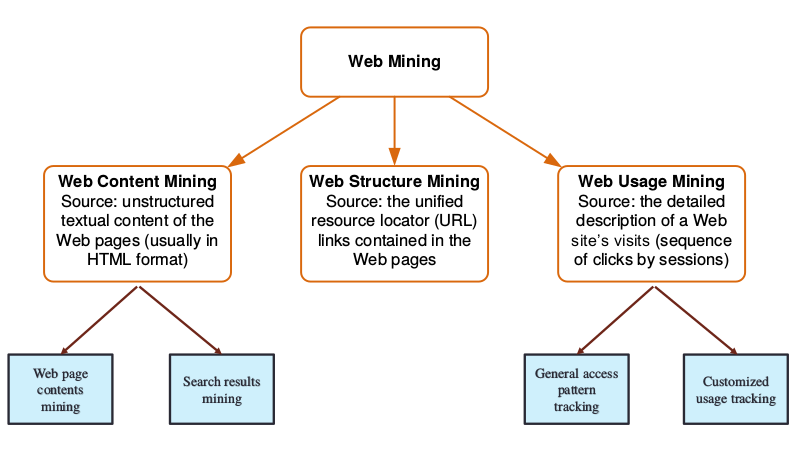
\includegraphics[width=0.7\textwidth]{figures/typed-of-webmining.png}
    \caption{dummy}
    \label{fig:XXX}
\end{figure}

\section{Conclusion}
\lipsum[20-30]

\section{References}
\bibliographystyle{ieeetr}
\renewcommand\refname{\vskip -1cm}
\bibliography{ST3012_project_report_v19pette_v18tobwe}

\end{document}
